\subsection{最短路径}
\begin{frame}\ft{\subsecname}
\begin{dingyi}
所谓最短路径,是指两点间经过的边上权值之和最小的路径。路径上的第一个顶点称为源点,最后一个顶点称为终点。
\end{dingyi}
\end{frame}

\begin{frame}\ft{\subsecname}
\begin{figure}
\centering
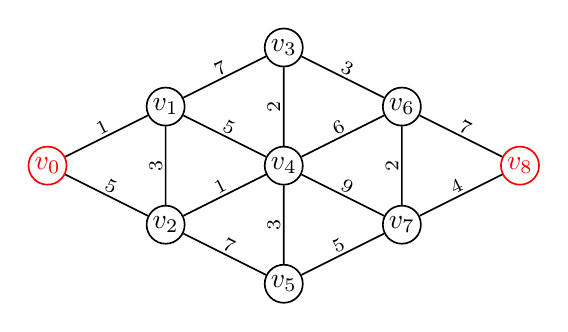
\begin{tikzpicture}[scale=1.5,node distance=1.5cm,semithick,inner sep=1pt,bend angle=45,sloped,anchor=south]
%\draw[help lines] (-3,-3) grid (3,0);
\node[circle,draw,red] (v0)  at(0,0)    {$v_0$};
\node[circle,draw] (v1)  at(1,0.5) {$v_1$};
\node[circle,draw] (v2)  at(1,-0.5) {$v_2$};
\node[circle,draw] (v3)  at(2,1) {$v_3$};
\node[circle,draw] (v4)  at(2,0) {$v_4$};
\node[circle,draw] (v5)  at(2,-1) {$v_5$};
\node[circle,draw] (v6)  at(3,0.5) {$v_6$};
\node[circle,draw] (v7)  at(3,-0.5) {$v_7$};
\node[circle,draw,red] (v8)  at(4,0) {$v_8$};
%%
\path
(v0) edge node{\scriptsize $1$} (v1)
     edge node{\scriptsize $5$} (v2)
(v1) edge node{\scriptsize $7$} (v3)
     edge node{\scriptsize $5$} (v4)
     edge node{\scriptsize $3$} (v2)
(v2) edge node{\scriptsize $1$} (v4)
     edge node{\scriptsize $7$} (v5)
(v3) edge node{\scriptsize $2$} (v4)
     edge node{\scriptsize $3$} (v6)
(v4) edge node{\scriptsize $6$} (v6)
     edge node{\scriptsize $9$} (v7)
     edge node{\scriptsize $3$} (v5)
(v5) edge node{\scriptsize $5$} (v7)
(v6) edge node{\scriptsize $2$} (v7)
     edge node{\scriptsize $7$} (v8)
(v7) edge node{\scriptsize $4$} (v8);  
      

\end{tikzpicture}

\end{figure}•

\end{frame}


\subsubsection{\tf Dijkstra算法}

\begin{frame}\ft{\subsubsecname}
\begin{figure}
\centering
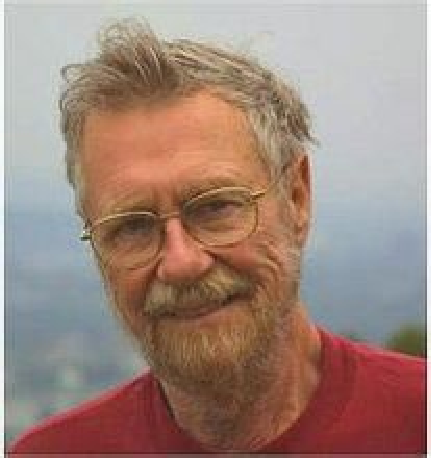
\includegraphics[width=1.5in]{Chapters/Ch06/Fig/dijkstra.pdf}
\caption{艾兹格·迪科斯彻(Edsger Wybe Dijkstr),1930-2002}
\end{figure}

荷兰人,计算机科学家。早年钻研物理及数学,而后转为计算机,1972年获得图灵奖。
\end{frame}

\begin{frame}\ft{\subsubsecname}
\tf Dijkstra算法是典型的单源最短路径算法,用于计算一个顶点到其他所有顶点的最短路径。
\vspace{0.1in}

\blue{主要特点:} 以起始点为中心向外层层扩展,直到扩展到终点为止。该算法要求图中不存在负权边。

\vspace{0.1in}

\blue{问题描述:} 在无向图G=(V,E)中,假设每条边$e_i$的长度为$w_i$,找到由顶点$v_0$到其余各点的最短路径(\red{单源最短路径})。
\end{frame}

\begin{frame}\ft{\subsubsecname}
\begin{block}{算法思想}
\tf设G=(V,E)是一个带权有向图,把图中顶点集合V分成两组。
\begin{itemize}
\item 第一组为已求出最短路径的顶点集合(用S表示,初始时S中只有一个源点,以后每求得一条最短路径,就将加入到集合S中,直到全部顶点都加入到S中,算法就结束)。\\[0.1in]
\item 第二组为其余未确定最短路径的顶点集合(用U表示),按最短路径长度的递增次序依次把第二组的顶点加入S中。在加入的过程中,总保持\blue{从源点v到S中各顶点的最短路径长度不大于从源点v到U中任何顶点的最短路径长度。}
\end{itemize}
此外,每个顶点对应一个距离,
\begin{itemize}
\item S中顶点的距离是从v到此顶点的最短路径长度
\item U中顶点的距离是从v到此顶点只包括S中顶点为中间顶点的当前最短路径长度。
\end{itemize}
\end{block}
\end{frame}

\begin{frame}\ft{\subsubsecname}
\begin{figure}
\centering
\begin{tikzpicture}[scale=1.5,node distance=1.5cm,semithick,inner sep=1pt,bend angle=45,sloped,anchor=south]
%\draw[help lines] (-3,-3) grid (3,0);
\node[circle,draw,red] (v0)  at(0,0)    {$v_0$};
\node[circle,draw,red] (v1)  at(1,0.5) {$v_1$};
\node[circle,draw] (v2)  at(1,-0.5) {$v_2$};
\node[circle,draw] (v3)  at(2,1) {$v_3$};
\node[circle,draw] (v4)  at(2,0) {$v_4$};
\node[circle,draw] (v5)  at(2,-1) {$v_5$};
\node[circle,draw] (v6)  at(3,0.5) {$v_6$};
\node[circle,draw] (v7)  at(3,-0.5) {$v_7$};
\node[circle,draw] (v8)  at(4,0) {$v_8$};
%%
\path
(v0) edge[->,>=latex',red] node{\scriptsize $1$} (v1)
     edgenode{\scriptsize $5$} (v2)
(v1) edge[->,>=latex',blue,dashed] node{\scriptsize $7$} (v3)
     edge[->,>=latex',blue,dashed]  node{\scriptsize $5$} (v4)
     edge[->,>=latex',red,dashed]  node{\scriptsize $3$} (v2)
(v2) edge node{\scriptsize $1$} (v4)
     edge node{\scriptsize $7$} (v5)
(v3) edge node{\scriptsize $2$} (v4)
     edge node{\scriptsize $3$} (v6)
(v4) edge node{\scriptsize $6$} (v6)
     edge node{\scriptsize $9$} (v7)
     edge node{\scriptsize $3$} (v5)
(v5) edge node{\scriptsize $5$} (v7)
(v6) edge node{\scriptsize $2$} (v7)
     edge node{\scriptsize $7$} (v8)
(v7) edge node{\scriptsize $4$} (v8);  
   
%\draw[->,>=latex',red] (v0)--(v1);   
%\draw[->,>=latex',red,dashed] (v1)--(v2);   
%\draw[->,>=latex',red,dashed] (v1)--(v3);   
%\draw[->,>=latex',red,dashed] (v1)--(v4);   

\end{tikzpicture}


\end{figure}

\begin{itemize}
\item
$v_0$到$v_1$的最短距离为$1$,路径为$v_0\to v_1$;\\[0.1in]
\item
由于$v_1$还与$v_2,v_3,v_4$连线,同时还可求得
$$
\begin{aligned}
&v_0\to v_1 \to v_2=1+3=4\\
&v_0\to v_1 \to v_3=1+7=8\\
&v_0\to v_1 \to v_4=1+5=6
\end{aligned}
$$

\end{itemize}•

\end{frame}

\begin{frame}\ft{\subsubsecname}
\begin{figure}
\centering
\begin{tikzpicture}[scale=1.5,node distance=1.5cm,semithick,inner sep=1pt,bend angle=45,sloped,anchor=south]
%\draw[help lines] (-3,-3) grid (3,0);
\node[circle,draw,red] (v0)  at(0,0)    {$v_0$};
\node[circle,draw,red] (v1)  at(1,0.5) {$v_1$};
\node[circle,draw,red] (v2)  at(1,-0.5) {$v_2$};
\node[circle,draw] (v3)  at(2,1) {$v_3$};
\node[circle,draw] (v4)  at(2,0) {$v_4$};
\node[circle,draw] (v5)  at(2,-1) {$v_5$};
\node[circle,draw] (v6)  at(3,0.5) {$v_6$};
\node[circle,draw] (v7)  at(3,-0.5) {$v_7$};
\node[circle,draw] (v8)  at(4,0) {$v_8$};
%%
\path
(v0) edge[->,>=latex',red] node{\scriptsize $1$} (v1)
     edgenode{\scriptsize $5$} (v2)
(v1) edge  node{\scriptsize $7$} (v3)
     edge  node{\scriptsize $5$} (v4)
     edge[->,>=latex',red]  node{\scriptsize $3$} (v2)
(v2) edge[->,>=latex',red,dashed] node{\scriptsize $1$} (v4)
     edge[->,>=latex',blue,dashed] node{\scriptsize $7$} (v5)
(v3) edge node{\scriptsize $2$} (v4)
     edge node{\scriptsize $3$} (v6)
(v4) edge node{\scriptsize $6$} (v6)
     edge node{\scriptsize $9$} (v7)
     edge node{\scriptsize $3$} (v5)
(v5) edge node{\scriptsize $5$} (v7)
(v6) edge node{\scriptsize $2$} (v7)
     edge node{\scriptsize $7$} (v8)
(v7) edge node{\scriptsize $4$} (v8);  
   
%\draw[->,>=latex',red] (v0)--(v1);   
%\draw[->,>=latex',red,dashed] (v1)--(v2);   
%\draw[->,>=latex',red,dashed] (v1)--(v3);   
%\draw[->,>=latex',red,dashed] (v1)--(v4);   

\end{tikzpicture}

\end{figure}

\begin{itemize}
\item
由于$v_0\to v_2=5$,比$v_0\to v_1 \to v_2=4$大,故$v_0$到$v_2$的最短距离为$4$;\\[0.1in]
\item
由于$v_2$还与$v_4,v_5$连线,同时还可求得
$$
\begin{aligned}
&\blue{v_0\to v_2} \to v_4=4+1=5\\
&\blue{v_0\to v_2} \to v_5=4+7=11
\end{aligned}
$$

\end{itemize}•

\end{frame}

\begin{frame}\ft{\subsubsecname}
\begin{figure}
\centering
\begin{tikzpicture}[scale=1.5,node distance=1.5cm,semithick,inner sep=1pt,bend angle=45,sloped,anchor=south]
%\draw[help lines] (-3,-3) grid (3,0);
\node[circle,draw,red] (v0)  at(0,0)    {$v_0$};
\node[circle,draw,red] (v1)  at(1,0.5) {$v_1$};
\node[circle,draw,red] (v2)  at(1,-0.5) {$v_2$};
\node[circle,draw] (v3)  at(2,1) {$v_3$};
\node[circle,draw] (v4)  at(2,0) {$v_4$};
\node[circle,draw] (v5)  at(2,-1) {$v_5$};
\node[circle,draw] (v6)  at(3,0.5) {$v_6$};
\node[circle,draw] (v7)  at(3,-0.5) {$v_7$};
\node[circle,draw] (v8)  at(4,0) {$v_8$};
%%
\path
(v0) edge[->,>=latex',red] node{\scriptsize $1$} (v1)
     edgenode{\scriptsize $5$} (v2)
(v1) edge  node{\scriptsize $7$} (v3)
     edge  node{\scriptsize $5$} (v4)
     edge[->,>=latex',red]  node{\scriptsize $3$} (v2)
(v2) edge[->,>=latex',red] node{\scriptsize $1$} (v4)
     edge node{\scriptsize $7$} (v5)
(v3) edge[<-,>=latex',red,dashed] node{\scriptsize $2$} (v4)
     edge node{\scriptsize $3$} (v6)
(v4) edge[->,>=latex',blue,dashed] node{\scriptsize $6$} (v6)
     edge[->,>=latex',blue,dashed] node{\scriptsize $9$} (v7)
     edge[->,>=latex',blue,dashed] node{\scriptsize $3$} (v5)
(v5) edge node{\scriptsize $5$} (v7)
(v6) edge node{\scriptsize $2$} (v7)
     edge node{\scriptsize $7$} (v8)
(v7) edge node{\scriptsize $4$} (v8);  
 

\end{tikzpicture}

\end{figure}

\begin{itemize}
\item
由于$v_0\to v_1\to v_4=6$,比$v_0\to v_1 \to v_2 \to v_4=5$大,故$v_0$到$v_4$的最短距离为$5$;\\[0.1in]
\item
由于$v_4$还与$v_3,v_5,v_6,v_7$连线,同时还可求得
$$
\begin{array}{ll}
 \blue{v_0\to v_4} \to v_3=5+2=7,   
&\blue{v_0\to v_4} \to v_5=5+3=8, \\
 \blue{v_0\to v_4} \to v_6=5+6=11,   
&\blue{v_0\to v_4} \to v_7=5+9=14.
\end{array}
$$

\end{itemize}•

\end{frame}

\begin{frame}\ft{\subsubsecname}
\begin{figure}
\centering
\begin{tikzpicture}[scale=1.5,node distance=1.5cm,semithick,inner sep=1pt,bend angle=45,sloped,anchor=south]
%\draw[help lines] (-3,-3) grid (3,0);
\node[circle,draw,red] (v0)  at(0,0)    {$v_0$};
\node[circle,draw,red] (v1)  at(1,0.5) {$v_1$};
\node[circle,draw,red] (v2)  at(1,-0.5) {$v_2$};
\node[circle,draw] (v3)  at(2,1) {$v_3$};
\node[circle,draw] (v4)  at(2,0) {$v_4$};
\node[circle,draw] (v5)  at(2,-1) {$v_5$};
\node[circle,draw] (v6)  at(3,0.5) {$v_6$};
\node[circle,draw] (v7)  at(3,-0.5) {$v_7$};
\node[circle,draw] (v8)  at(4,0) {$v_8$};
%%
\path
(v0) edge[->,>=latex',red] node{\scriptsize $1$} (v1)
     edgenode{\scriptsize $5$} (v2)
(v1) edge  node{\scriptsize $7$} (v3)
     edge  node{\scriptsize $5$} (v4)
     edge[->,>=latex',red]  node{\scriptsize $3$} (v2)
(v2) edge[->,>=latex',red] node{\scriptsize $1$} (v4)
     edge node{\scriptsize $7$} (v5)
(v3) edge[<-,>=latex',red] node{\scriptsize $2$} (v4)
     edge node{\scriptsize $3$} (v6)
(v4) edge node{\scriptsize $6$} (v6)
     edge  node{\scriptsize $9$} (v7)
     edge  node{\scriptsize $3$} (v5)
(v5) edge node{\scriptsize $5$} (v7)
(v6) edge node{\scriptsize $2$} (v7)
     edge node{\scriptsize $7$} (v8)
(v7) edge node{\scriptsize $4$} (v8);  
 

\end{tikzpicture}

\end{figure}

\begin{itemize}
\item
由于$v_0\to v_1\to v_3=8$,比$v_0\to v_1 \to v_2 \to v_4 \to v_3=7$大,故$v_0$到$v_3$的最短距离为$7$;\\[0.1in]
%\item
%由于$v_3$还与$v_6$连线,同时还可求得
%$$
%\begin{array}{ll}
% \blue{v_0\to v_3} \to v_6=7+3=10.
%\end{array}
%$$

\end{itemize}•
\end{frame}




\begin{frame}\ft{\subsubsecname}
\tf Dijkstra算法并不是一下子就求出$v_0$到$v_8$的最短路径,而是一步步求出它们之间顶点的最短路径,过程中在已经求出的最短路径的基础上,再求得更远顶点的最短路径,最终得到想要的结果。
\end{frame}


\begin{frame}\ft{\subsubsecname}
\lstinputlisting[
language=c,
numbers=left,
numberstyle=\tiny,
frame=tb,
]{Chapters/Ch06/Code/adjmatrix/adjmatrix.h}
\end{frame}



\begin{frame}\ft{\subsubsecname}
\lstinputlisting[
language=c,
linerange={121-131},
numbers=left,
numberstyle=\tiny,
frame=tb,
]{Chapters/Ch06/Code/adjmatrix/adjmatrix.c}
\end{frame}


\begin{frame}\ft{\subsubsecname}
\lstinputlisting[
language=c,
linerange={133-149},
numbers=left,
firstnumber=12,
numberstyle=\tiny,
frame=tb,
]{Chapters/Ch06/Code/adjmatrix/adjmatrix.c}
\end{frame}



\begin{frame}[fragile]\ft{\subsubsecname} 
\begin{figure}
\centering
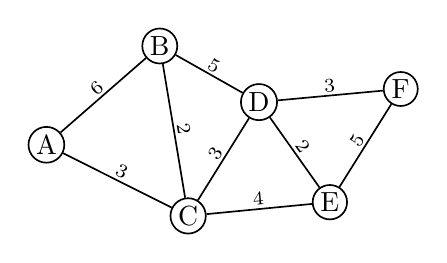
\begin{tikzpicture}[scale=1.8,node distance=1.5cm,semithick,inner sep=1pt,bend angle=45,sloped,anchor=south]
%\draw[help lines] (-3,-3) grid (3,0);
\node[circle,draw] (A)  at(0,0)    {A};
\node[circle,draw] (B)  at(0.8,0.7) {B};
\node[circle,draw] (C)  at(1,-0.5) {C};
\node[circle,draw] (D)  at(1.5,0.3) {D};
\node[circle,draw] (E)  at(2,-0.4) {E};
\node[circle,draw] (F)  at(2.5,0.4) {F}; 

\path
(A)  edge node{\scriptsize $6$} (B)
     edge node{\scriptsize $3$} (C)
(B)  edge node{\scriptsize $2$} (C)
     edge node{\scriptsize $5$} (D)
(C)  edge node{\scriptsize $3$} (D)
     edge node{\scriptsize $4$} (E)
(D)  edge node{\scriptsize $2$} (E)
     edge node{\scriptsize $3$} (F)
(E)  edge node{\scriptsize $5$} (F);  
 

\end{tikzpicture}

\end{figure}

\end{frame}



\begin{frame}[fragile]\ft{\subsubsecname} 
\begin{small}
\begin{table}
\centering
\begin{tabular}{|l|l|l|}\hline
步骤&\tf 集合S中 &\tf 集合U中\\\hline
1
&\tf 选入A,S=<A>
&\tf U=<B,C,D,E,F>\\
&\tf 此时最短路径为A$\to$A=0
&\tf A$\to$B=6\\
&\tf 从A开始找&\tf A$\to$C=3\\
&
&\tf A$\to$U中其他顶点=$\infty$\\
&
&\tf 发现A$\to$C=3权值最小\\\hline
\end{tabular}
\end{table}
\end{small}
\end{frame}


\begin{frame}[fragile]\ft{\subsubsecname} 
\begin{small}
\begin{table}
\centering
\begin{tabular}{|l|l|l|}\hline
步骤&\tf 集合S中 &\tf 集合U中\\\hline
2&\tf 选入C,S=<A,C>
&\tf U=<B,D,E,F>\\
&\tf 最短路径为
&\tf A$\to$C$\to$B=5\\
&\tf A$\to$A=0, A$\to$C=3
&\tf A$\to$C$\to$D=6\\
&\tf 从路径A$\to$C开始找
&\tf A$\to$C$\to$E=7\\
&
&\tf A$\to$C$\to$U中其他顶点=$\infty$\\
&
&\tf发现A$\to$C$\to$B=5权值最小\\\hline
\end{tabular}
\end{table}
\end{small}
\end{frame}

\begin{frame}[fragile]\ft{\subsubsecname} 
\begin{small}
\begin{table}
\centering
\begin{tabular}{|l|l|l|}\hline
步骤&\tf 集合S中 &\tf 集合U中\\\hline
3&\tf 选入B,S=<A,C,B>,最短路径为
&\tf U=<D,E,F>\\
&\tf A$\to$A=0, A$\to$C=3, A$\to$C$\to$B=5,
&\tf A$\to$C$\to$B$\to$D=10, \\
&\tf 从路径A$\to$C$\to$B开始找.
&\tf 比第二步的A$\to$C$\to$D=6要长,\\
&\tf 
&\tf 到D权值改为A$\to$C$\to$D=6;\\
&\tf 
&\tf A$\to$C$\to$B$\to$U中其他顶点=$\infty$;\\
&
&\tf 发现A$\to$C$\to$D=6权值最小. \\\hline
\end{tabular}
\end{table}
\end{small}
\end{frame}


\begin{frame}[fragile]\ft{\subsubsecname} 
\begin{small}
\begin{table}
\centering
\begin{tabular}{|l|l|l|}\hline
步骤&\tf 集合S中 &\tf 集合U中\\\hline
4&\tf 选入D,S=<A,C,B,D>,最短路径为
&\tf U=<E,F>\\
&\tf A$\to$A=0, A$\to$C=3,
&\tf A$\to$C$\to$D$\to$E=8, \\
&\tf A$\to$C$\to$B=5, A$\to$C$\to$D=6
&\tf 比第二步的A$\to$C$\to$E=7要长,\\
&\tf 从路径A$\to$C$\to$D开始找
&\tf 到E权值改为A$\to$C$\to$E=7;\\
&\tf 
&\tf A$\to$C$\to$D$\to$F=9;\\
&
&\tf 发现A$\to$C$\to$E=7权值最小.\\\hline
\end{tabular}
\end{table}
\end{small}
\end{frame}

\begin{frame}[fragile]\ft{\subsubsecname} 
\begin{small}
\begin{table}
\centering
\begin{tabular}{|l|l|l|}\hline
步骤&\tf 集合S中 &\tf 集合U中\\\hline
5&\tf 选入E,S=<A,C,B,D,E>,最短路径为
&\tf U=<F>\\
&\tf A$\to$A=0, A$\to$C=3,
&\tf A$\to$C$\to$E$\to$F=12, \\
&\tf A$\to$C$\to$B=5, A$\to$C$\to$D=6
&\tf 比第四步的A$\to$C$\to$D$\to$F=9长,\\
&\tf A$\to$C$\to$E=7,
&\tf 到F权值改为A$\to$C$\to$F=9;\\
&\tf 从路径A$\to$C$\to$E开始找
&\tf 发现A$\to$C$\to$D$\to$F=9权值最小. \\\hline
\end{tabular}
\end{table}
\end{small}
\end{frame}

\begin{frame}[fragile]\ft{\subsubsecname} 
\begin{small}
\begin{table}
\centering
\begin{tabular}{|l|l|l|}\hline
步骤&\tf 集合S中 &\tf 集合U中\\\hline
6&\tf 选入F,S=<A,C,B,D,E,F>,最短路径为
&\tf U=<>, 查找完毕\\
&\tf A$\to$A=0,  A$\to$C=3,
&\tf   \\
&\tf A$\to$C$\to$B=5, A$\to$C$\to$D=6
&\tf  \\
&\tf A$\to$C$\to$E=7, A$\to$C$\to$D$\to$F=9.
&\tf  \\\hline
\end{tabular}
\end{table}
\end{small}
\end{frame}



\begin{frame}[fragile]\ft{\subsubsecname}\fst{程序详解}
\begin{figure}
\centering
\begin{tikzpicture}[scale=1.8,node distance=1.5cm,semithick,inner sep=1pt,bend angle=45,sloped,anchor=south]
%\draw[help lines] (-3,-3) grid (3,0);
\node[circle,draw] (A)  at(0,0)    {A};
\node[circle,draw] (B)  at(0.8,0.7) {B};
\node[circle,draw] (C)  at(1,-0.5) {C};
\node[circle,draw] (D)  at(1.5,0.3) {D};
\node[circle,draw] (E)  at(2,-0.4) {E};
\node[circle,draw] (F)  at(2.5,0.4) {F}; 

\path
(A)  edge node{\scriptsize $6$} (B)
     edge node{\scriptsize $3$} (C)
(B)  edge node{\scriptsize $2$} (C)
     edge node{\scriptsize $5$} (D)
(C)  edge node{\scriptsize $3$} (D)
     edge node{\scriptsize $4$} (E)
(D)  edge node{\scriptsize $2$} (E)
     edge node{\scriptsize $3$} (F)
(E)  edge node{\scriptsize $5$} (F);  
 
\matrix (d) at (1.5,-2.5) [matrix of math nodes,left delimiter=(,right delimiter=),row sep=5pt,column sep=5pt] 
  {
    0 & 6 & 3 & \infty & \infty & \infty    \\    
    6 & 0 & 2 & 5 & \infty & \infty \\
    3 & 2 & 0 & 3 & 4 & \infty \\
    \infty & 5 & 3 & 0 & 2 & 3 \\
    \infty & \infty  &  4 & 2 & 0 & 5 \\
    \infty & \infty & \infty & 3 & 5 & 0 \\ 
      };
      
      
\end{tikzpicture}




\end{figure}
\end{frame}



\begin{frame}[fragile]\ft{\subsubsecname}\fst{程序详解}

\tf初始化(从A(v0=0)开始)
\lstinputlisting[
language=c,
linerange={125-131},
numbers=left,
firstnumber=5,
numberstyle=\tiny,
frame=tb,
]{Chapters/Ch06/Code/adjmatrix/adjmatrix.c}

\begin{lstlisting}
dist={0,6,3,INF,INF,INF}
prev={0,0,0,0,0,0}
S={1,0,0,0,0,0}
\end{lstlisting}

\end{frame}


\begin{frame}[fragile]\ft{\subsubsecname}\fst{程序详解}

\tf 第一次循环(v=1) 
\begin{lstlisting}
S   ={1,0,0,0,0,0}
dist={0,6,3,INF,INF,INF}
\end{lstlisting}


\lstinputlisting[
language=c,
linerange={134-141},
numbers=left,
firstnumber=13,
numberstyle=\tiny,
frame=tb,
]{Chapters/Ch06/Code/adjmatrix/adjmatrix.c}

%\pause 
\begin{lstlisting}
min=3, k=2.
S={1,0,1,0,0,0}
\end{lstlisting}

\end{frame}


\begin{frame}[fragile]\ft{\subsubsecname}\fst{程序详解}

\tf 第一次循环(v=1)
\begin{lstlisting}
min=3, k=2.
S   ={1,0,1,0,0,0}
dist={0,6,3,INF,INF,INF}
prev={0,0,0,0,0,0}
\end{lstlisting}

\lstinputlisting[
language=c,
linerange={142-147},
numbers=left,
firstnumber=21,
numberstyle=\tiny,
frame=tb,
]{Chapters/Ch06/Code/adjmatrix/adjmatrix.c}
%\pause 

\begin{lstlisting}
dist={0,5,3,6,7,INF}
prev={0,2,0,2,2,0}
\end{lstlisting}

\end{frame}

\begin{frame}[fragile]\ft{\subsubsecname}\fst{程序详解}

\tf 第二次循环(v=2) 
\begin{lstlisting}
S   ={1,0,1,0,0,0}
dist={0,5,3,6,7,INF}
\end{lstlisting}

\lstinputlisting[
language=c,
linerange={134-141},
numbers=left,
firstnumber=13,
numberstyle=\tiny,
frame=tb,
]{Chapters/Ch06/Code/adjmatrix/adjmatrix.c}

%\pause 
\begin{lstlisting}
min=5, k=1
S={1,1,1,0,0,0}
\end{lstlisting}

\end{frame}


\begin{frame}[fragile]\ft{\subsubsecname}\fst{程序详解}

\tf 第二次循环(v=2)
\begin{lstlisting}
min=5, k=1
S   ={1,1,1,0,0,0}
dist={0,5,3,6,7,INF}
prev={0,2,0,2,2,0}
\end{lstlisting}
 
\lstinputlisting[
language=c,
linerange={142-147},
numbers=left,
firstnumber=21,
numberstyle=\tiny,
frame=tb,
]{Chapters/Ch06/Code/adjmatrix/adjmatrix.c}

%\pause 
\begin{lstlisting}
dist={0,5,3,6,7,INF}
prev={0,2,0,2,2,0}
\end{lstlisting}

\end{frame}


\begin{frame}[fragile]\ft{\subsubsecname}\fst{程序详解}

\tf 第三次循环(v=3) 
\begin{lstlisting}
S   ={1,1,1,0,0,0}
dist={0,5,3,6,7,INF}
\end{lstlisting}

\lstinputlisting[
language=c,
linerange={134-141},
numbers=left,
firstnumber=13,
numberstyle=\tiny,
frame=tb,
]{Chapters/Ch06/Code/adjmatrix/adjmatrix.c}

%\pause 
\begin{lstlisting}
min=6, k=3
S={1,1,1,1,0,0}
\end{lstlisting}

\end{frame}


\begin{frame}[fragile]\ft{\subsubsecname}\fst{程序详解}

\tf 第三次循环(v=3)
\begin{lstlisting}
min=6, k=3
S   ={1,1,1,1,0,0}
dist={0,5,3,6,7,INF}
prev={0,2,0,2,2,0}
\end{lstlisting}
 
\lstinputlisting[
language=c,
linerange={142-147},
numbers=left,
firstnumber=21,
numberstyle=\tiny,
frame=tb,
]{Chapters/Ch06/Code/adjmatrix/adjmatrix.c}

%\pause 
\begin{lstlisting}
dist={0,5,3,6,7,9}
prev={0,2,0,2,2,3}
\end{lstlisting}

\end{frame}


\begin{frame}[fragile]\ft{\subsubsecname}\fst{程序详解}

\tf 第四次循环(v=4) 
\begin{lstlisting}
S   ={1,1,1,1,0,0}
dist={0,5,3,6,7,9}
\end{lstlisting}

\lstinputlisting[
language=c,
linerange={134-141},
numbers=left,
firstnumber=13,
numberstyle=\tiny,
frame=tb,
]{Chapters/Ch06/Code/adjmatrix/adjmatrix.c}

%\pause 
\begin{lstlisting}
min=7, k=4
S={1,1,1,1,1,0}
\end{lstlisting}

\end{frame}


\begin{frame}[fragile]\ft{\subsubsecname}\fst{程序详解}

\tf 第四次循环(v=4) 
\begin{lstlisting}
min=7, k=4
S   ={1,1,1,1,1,0}
dist={0,5,3,6,7,9}
prev={0,2,0,2,2,3}
\end{lstlisting}
 
\lstinputlisting[
language=c,
linerange={142-147},
numbers=left,
firstnumber=21,
numberstyle=\tiny,
frame=tb,
]{Chapters/Ch06/Code/adjmatrix/adjmatrix.c}

%\pause 
\begin{lstlisting}
dist={0,5,3,6,7,9}
prev={0,2,0,2,2,3}
\end{lstlisting}

\end{frame}


\begin{frame}[fragile]\ft{\subsubsecname}\fst{程序详解}

\tf 第五次循环(v=5) 
\begin{lstlisting}
S   ={1,1,1,1,1,0}
dist={0,5,3,6,7,9}
\end{lstlisting}

\lstinputlisting[
language=c,
linerange={134-141},
numbers=left,
firstnumber=13,
numberstyle=\tiny,
frame=tb,
]{Chapters/Ch06/Code/adjmatrix/adjmatrix.c}

%\pause 
\begin{lstlisting}
min=9, k=5
S={1,1,1,1,1,1}
\end{lstlisting}

\end{frame}

\begin{frame}[fragile]\ft{\subsubsecname}\fst{程序详解}

\tf 第五次循环(v=5) 
\begin{lstlisting}
min=9, k=5
S   ={1,1,1,1,1,1}
//`表示所有的顶点均完成了最短路径的查找工作`

dist={0,5,3,6,7,9}
//`表示`v0`到各顶点的最短路径数,如`dist[4]=7

prev={0,2,0,2,2,3}
//`表示各顶点的前驱`
//prev[4]=2: E`的前驱为`C
//prev[2]=0: C`的前驱为`A
//`故`A`到`E`的最短路径为`A=>C=>E
\end{lstlisting}


\end{frame}



 
%
%\begin{frame}\ft{\subsubsecname}\fst{程序详解}
%\begin{figure}
%\centering
%\begin{tikzpicture}[scale=1.5,node distance=1.5cm,semithick,inner sep=1pt,bend angle=45,sloped,anchor=south]
%\draw[help lines] (-3,-3) grid (3,0);
\node[circle,draw,red] (v0)  at(0,0)    {$v_0$};
\node[circle,draw,red] (v1)  at(1,0.5) {$v_1$};
\node[circle,draw,red] (v2)  at(1,-0.5) {$v_2$};
\node[circle,draw] (v3)  at(2,1) {$v_3$};
\node[circle,draw] (v4)  at(2,0) {$v_4$};
\node[circle,draw] (v5)  at(2,-1) {$v_5$};
\node[circle,draw] (v6)  at(3,0.5) {$v_6$};
\node[circle,draw] (v7)  at(3,-0.5) {$v_7$};
\node[circle,draw] (v8)  at(4,0) {$v_8$};
%%
\path
(v0) edge[->,>=latex',red] node{\scriptsize $1$} (v1)
     edgenode{\scriptsize $5$} (v2)
(v1) edge  node{\scriptsize $7$} (v3)
     edge  node{\scriptsize $5$} (v4)
     edge[->,>=latex',red]  node{\scriptsize $3$} (v2)
(v2) edge[->,>=latex',red] node{\scriptsize $1$} (v4)
     edge node{\scriptsize $7$} (v5)
(v3) edge[<-,>=latex',red] node{\scriptsize $2$} (v4)
     edge[->,>=latex',red] node{\scriptsize $3$} (v6)
(v4) edge node{\scriptsize $6$} (v6)
     edge  node{\scriptsize $9$} (v7)
     edge  node{\scriptsize $3$} (v5)
(v5) edge node{\scriptsize $5$} (v7)
(v6) edge[->,>=latex',red] node{\scriptsize $2$} (v7)
     edge node{\scriptsize $7$} (v8)
(v7) edge[->,>=latex',red] node{\scriptsize $4$} (v8);  
 

\end{tikzpicture}

%\end{figure}
%
%\end{frame}


\subsubsection{\tf Floyd算法}


\begin{frame}\ft{\subsubsecname}
\begin{figure}
\centering
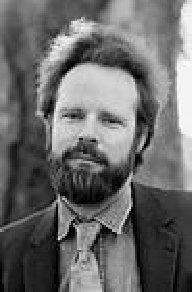
\includegraphics[width=1in]{Chapters/Ch06/Fig/floyd}
\caption{罗伯特·弗洛伊德(Robert W.Floyd),1936-2001}
\end{figure}
美国人,计算机科学家。1953年芝加哥大学获得文学学士学位,1978年获得图灵奖。
\end{frame}




\begin{frame}\ft{\subsubsecname}
\tf \blue{算法思想:} Floyd算法是一个经典的动态规划算法,目标是寻找从点i到点j的最短路径。
\vspace{0.1in}

从任意顶点i到任意顶点j的最短路径不外乎2种可能:
\begin{itemize}
\item 从i直接到j,
\item 从i经过若干个顶点k到j.
\end{itemize}
\end{frame}




\begin{frame}[fragile]\ft{\subsubsecname}
\tf 设dist(i,j)为顶点i到顶点j的最短路径的距离。对于每一个顶点k,检查
\begin{lstlisting}
dist(i,k)+dist(k,j)<dist(i,j)
\end{lstlisting}
是否成立。若成立,说明从i到k再到j的路径比i直接到j的路径短,设置
\begin{lstlisting}
dist(i,j)=dist(i,k)+dist(k,j).
\end{lstlisting}
于是,当我们遍历完所有节点k,dist(i,j)中记录的便是i到j的最短路径的距离。


\end{frame}


\begin{frame}\ft{\subsubsecname}
\tf \blue{算法描述:}  

\begin{itemize}
\item \tf 从任意一条单边路径开始。所有两点之间的距离是边的权,如果两点之间没有边相连,则权为INF。\\[0.1in]
\item \tf 对于每一对顶点u和v,看看是否存在一个顶点w使得从u到w再到v比己知的路径更短。如果是更新它。
\end{itemize}
\end{frame}

\begin{frame}\ft{\subsubsecname}
\begin{figure}
\centering
\begin{tikzpicture}[scale=0.9,node distance=2cm,semithick,inner sep=1pt,bend angle=45,sloped]
%\draw[help lines] (-3,-3) grid (3,0);
\node[circle,draw] (v1)  at (0,0)   {$v_1$};
\node[circle,draw] (v2)  at (2,0) {$v_2$};
\node[circle,draw] (v0) at (1,1.732) {$v_0$};
 
%%
\path
(v0) edge node{\small $2$} (v1)
     edge node{\small $1$} (v2)
(v1) edge node{\small $5$} (v2);  
 
       
\matrix (dm) at (4,1.5) [matrix of math nodes,left delimiter=(,right delimiter=),row sep=5pt,column sep=5pt,right] 
  {
    0 & 2& 1\\
    2& 0 & 5 \\
    1& 5&  0\\
  };
  \node at (dm-1-1) [above left=15pt] {$D^{(-1)}$}; 
  \node at (dm-1-1) [above=10pt] {$\small v_0$}; 
  \node at (dm-1-2) [above=10pt] {$\small v_1$};       
  \node at (dm-1-3) [above=10pt] {$\small v_2$};   
  \node at (dm-1-1) [left=18pt] {$\small v_0$}; 
  \node at (dm-2-1) [left=18pt] {$\small v_1$};       
  \node at (dm-3-1) [left=18pt] {$\small v_2$};   
  
  \matrix (d0) at (7.5,1.5)  [matrix of math nodes]
  {
  \xlongrightarrow[{\therefore~ D^{(-1)}[1][2]=\atop D^{(-1)}[1][0]+D^{-1}[0][2]}]{\because~ D^{(-1)}[1][2]>\atop D^{(-1)}[1][0]+D^{(-1)}[0][2]}\\
  };
\matrix (d0) at (10.5,1.5) [matrix of math nodes,left delimiter=(,right delimiter=),row sep=5pt,column sep=5pt,right] 
  {
    0 & 2& 1\\
    2& 0 & 3 \\
    1& 3&  0\\
  };
  \node at (d0-1-1) [above left=15pt] {$D^{(0)}$}; 
  \node at (d0-1-1) [above=10pt] {$\small v_0$}; 
  \node at (d0-1-2) [above=10pt] {$\small v_1$};       
  \node at (d0-1-3) [above=10pt] {$\small v_2$};   
  \node at (d0-1-1) [left=18pt] {$\small v_0$}; 
  \node at (d0-2-1) [left=18pt] {$\small v_1$};       
  \node at (d0-3-1) [left=18pt] {$\small v_2$};       
  
  \matrix (pm) at (4,-1.2)  [matrix of math nodes,left delimiter=(,right delimiter=),row sep=5pt,column sep=5pt,right] 
  {
    0 & 1& 2\\
    0 & 1& 2 \\
    0 & 1& 2\\
  };
    \node at (pm-1-1) [above left=15pt] {$P^{(-1)}$}; 
  \node at (pm-1-1) [above=10pt] {$\small v_0$}; 
  \node at (pm-1-2) [above=10pt] {$\small v_1$};       
  \node at (pm-1-3) [above=10pt] {$\small v_2$};   
  \node at (pm-1-1) [left=18pt] {$\small v_0$}; 
  \node at (pm-2-1) [left=18pt] {$\small v_1$};       
  \node at (pm-3-1) [left=18pt] {$\small v_2$};       
      
  \matrix (d0) at (7.5,-1.2)  [matrix of math nodes]
  {
  \xlongrightarrow[]{}\\
  };
  
  \matrix (p0) at (10.5,-1.2)  [matrix of math nodes,left delimiter=(,right delimiter=),row sep=5pt,column sep=5pt,right] 
  {
    0 & 1& 2\\
    0 & 1& 0 \\
    0 & 0& 2\\
  };
    \node at (p0-1-1) [above left=15pt] {$P^{(0)}$}; 
  \node at (p0-1-1) [above=10pt] {$\small v_0$}; 
  \node at (p0-1-2) [above=10pt] {$\small v_1$};       
  \node at (p0-1-3) [above=10pt] {$\small v_2$};   
  \node at (p0-1-1) [left=18pt] {$\small v_0$}; 
  \node at (p0-2-1) [left=18pt] {$\small v_1$};       
  \node at (p0-3-1) [left=18pt] {$\small v_2$}; 
\end{tikzpicture}

\end{figure}
\end{frame}

\begin{frame}\ft{\subsubsecname}
\tf 先定义两个数组
\begin{itemize}
\item D[3][3]:表示顶点到顶点的最短路径权值和的矩阵,其初始值就为图的邻接矩阵。\\[0.1in]
\item P[3][3]:表示对应顶点的最小路径的前驱矩阵,其初始值如图所示。
\end{itemize}•
\end{frame}

\begin{frame}[fragile]\ft{\subsubsecname}
分析所有的顶点经过$v_0$后到达另一顶点的最短路径。
\begin{itemize}
\item 查看路径$v_1\to v_0\to v_2$,得到
\begin{lstlisting}[mathescape]
D$^{(-1)}$[1][0]+D$^{(-1)}$[0][2]=2+1=3.
\end{lstlisting}
\item 查看路径$v_1\to  v_2$,得到
\begin{lstlisting}[mathescape]
D$^{(-1)}$[1][2]=5.
\end{lstlisting}
\item 因为
\begin{lstlisting}[mathescape]
D$^{(-1)}$[1][2] > D$^{(-1)}$[1][0]+D$^{(-1)}$[0][2] 
\end{lstlisting}
即$v_1\to v_0\to v_2$比$v_1\to  v_2$更近,就让
\begin{lstlisting}[mathescape]
D$^{(-1)}$[1][2] = D$^{(-1)}$[2][1] 
           = D$^{(-1)}$[1][0]+D$^{(-1)}$[0][2].
\end{lstlisting}
\tf矩阵P中的P$^{(-1)}$[1][2]和P$^{(-1)}$[2][1]也修改为当前中转顶点$v_0$的下标0。
\end{itemize}

\end{frame}





\begin{frame}[fragile]\ft{\subsubsecname}
\begin{lstlisting}[mathescape]
D$^{(0)}$[v][w]=min{D$^{(-1)}$[v][w], D$^{(-1)}$[v][0]+D$^{(-1)}$[0][w]}
\end{lstlisting}
\end{frame}




\begin{frame}\ft{\subsubsecname}
\begin{figure}
\centering
\begin{tikzpicture}[scale=1.2,node distance=2cm,semithick,inner sep=1pt,bend angle=45,sloped,anchor=south]
%\draw[help lines] (-3,-3) grid (3,0);
\node[circle,draw] (v0)  at(0,0)    {$v_0$};
\node[circle,draw] (v1)  at(1,0.5) {$v_1$};
\node[circle,draw] (v2)  at(1,-0.5) {$v_2$};
\node[circle,draw] (v3)  at(2,1) {$v_3$};
\node[circle,draw] (v4)  at(2,0) {$v_4$};
\node[circle,draw] (v5)  at(2,-1) {$v_5$};
\node[circle,draw] (v6)  at(3,0.5) {$v_6$};
\node[circle,draw] (v7)  at(3,-0.5) {$v_7$};
\node[circle,draw] (v8)  at(4,0) {$v_8$};
%%
\path
(v0) edge node{\scriptsize $1$} (v1)
     edge node{\scriptsize $5$} (v2)
(v1) edge node{\scriptsize $7$} (v3)
     edge node{\scriptsize $5$} (v4)
     edge node{\scriptsize $3$} (v2)
(v2) edge node{\scriptsize $1$} (v4)
     edge node{\scriptsize $7$} (v5)
(v3) edge node{\scriptsize $2$} (v4)
     edge node{\scriptsize $3$} (v6)
(v4) edge node{\scriptsize $6$} (v6)
     edge node{\scriptsize $9$} (v7)
     edge node{\scriptsize $3$} (v5)
(v5) edge node{\scriptsize $5$} (v7)
(v6) edge node{\scriptsize $2$} (v7)
     edge node{\scriptsize $7$} (v8)
(v7) edge node{\scriptsize $4$} (v8);  
      
     
\matrix (d) at (0,-4.4) [matrix of math nodes,left delimiter=(,right delimiter=),row sep=4pt,column sep=2pt] 
  {
    0 & 1 & 5 & \infty & \infty & \infty & \infty & \infty & \infty   \\
    1 & 0 & 3 & 7 & 5 & \infty & \infty & \infty & \infty \\ 
    5 & 3 & 0 & \infty & 1 & 7 & \infty & \infty & \infty   \\
    \infty & 7 & \infty & 0 & 2 & \infty & 3 & \infty & \infty \\ 
    \infty & 5 & 1 & 2 & 0 & 3 & 6 & 9 & \infty   \\
    \infty & \infty & 7 & \infty & 3 & 0 & \infty & 5 & \infty \\ 
    \infty & \infty & \infty & 3 & 6 & \infty & 0 & 2 & 7   \\
    \infty & \infty & \infty & \infty & 9 & 5 & 2 & 0 & 4 \\     
    \infty & \infty & \infty & \infty & \infty & \infty & 7 & 4 & 0 \\     
      };
  \node at (d-9-5) [below=4pt]{$D^{(-1)}$};
  
\matrix (p) at (4,-4.4) [matrix of math nodes,left delimiter=(,right delimiter=),row sep=4pt,column sep=2pt] 
  {
    0 & 1 & 2 & 3 & 4 & 5 & 6 & 7 & 8   \\
    0 & 1 & 2 & 3 & 4 & 5 & 6 & 7 & 8   \\
    0 & 1 & 2 & 3 & 4 & 5 & 6 & 7 & 8   \\
    0 & 1 & 2 & 3 & 4 & 5 & 6 & 7 & 8   \\                  
    0 & 1 & 2 & 3 & 4 & 5 & 6 & 7 & 8   \\
    0 & 1 & 2 & 3 & 4 & 5 & 6 & 7 & 8   \\
    0 & 1 & 2 & 3 & 4 & 5 & 6 & 7 & 8   \\
    0 & 1 & 2 & 3 & 4 & 5 & 6 & 7 & 8   \\
    0 & 1 & 2 & 3 & 4 & 5 & 6 & 7 & 8   \\  
 };   
    \node at (p-9-5) [below=4pt]{$P^{(-1)}$};
\end{tikzpicture}



\end{figure}
\end{frame}


\begin{frame}\ft{\subsubsecname}
\lstinputlisting[
language=c,
linerange={152-160},
numbers=left,
firstnumber=21,
numberstyle=\tiny,
frame=tb,
]{Chapters/Ch06/Code/adjmatrix/adjmatrix.c}
\end{frame}

\begin{frame}\ft{\subsubsecname}
\lstinputlisting[
language=c,
linerange={161-172},
numbers=left,
firstnumber=21,
numberstyle=\tiny,
frame=tb,
]{Chapters/Ch06/Code/adjmatrix/adjmatrix.c}
\end{frame}

\begin{frame}\ft{\subsubsecname}
\begin{figure}
\centering
\begin{tikzpicture}[scale=1.2,node distance=2cm,semithick,inner sep=1pt,bend angle=45,sloped,anchor=south]
%\draw[help lines] (-3,-3) grid (3,0);
\node[circle,draw,red] (v0)  at(0,0)    {$v_0$};
\node[circle,draw] (v1)  at(1,0.5) {$v_1$};
\node[circle,draw] (v2)  at(1,-0.5) {$v_2$};
\node[circle,draw] (v3)  at(2,1) {$v_3$};
\node[circle,draw] (v4)  at(2,0) {$v_4$};
\node[circle,draw] (v5)  at(2,-1) {$v_5$};
\node[circle,draw] (v6)  at(3,0.5) {$v_6$};
\node[circle,draw] (v7)  at(3,-0.5) {$v_7$};
\node[circle,draw] (v8)  at(4,0) {$v_8$};
%%
\path
(v0) edge node{\scriptsize $1$} (v1)
     edge node{\scriptsize $5$} (v2)
(v1) edge node{\scriptsize $7$} (v3)
     edge node{\scriptsize $5$} (v4)
     edge node{\scriptsize $3$} (v2)
(v2) edge node{\scriptsize $1$} (v4)
     edge node{\scriptsize $7$} (v5)
(v3) edge node{\scriptsize $2$} (v4)
     edge node{\scriptsize $3$} (v6)
(v4) edge node{\scriptsize $6$} (v6)
     edge node{\scriptsize $9$} (v7)
     edge node{\scriptsize $3$} (v5)
(v5) edge node{\scriptsize $5$} (v7)
(v6) edge node{\scriptsize $2$} (v7)
     edge node{\scriptsize $7$} (v8)
(v7) edge node{\scriptsize $4$} (v8);  
      
     
\matrix (d) at (0,-4.4) [matrix of math nodes,left delimiter=(,right delimiter=),row sep=4pt,column sep=2pt] 
  {
    0 & 1 & 5 & \infty & \infty & \infty & \infty & \infty & \infty   \\
    1 & 0 & 3 & 7 & 5 & \infty & \infty & \infty & \infty \\ 
    5 & 3 & 0 & \infty & 1 & 7 & \infty & \infty & \infty   \\
    \infty & 7 & \infty & 0 & 2 & \infty & 3 & \infty & \infty \\ 
    \infty & 5 & 1 & 2 & 0 & 3 & 6 & 9 & \infty   \\
    \infty & \infty & 7 & \infty & 3 & 0 & \infty & 5 & \infty \\ 
    \infty & \infty & \infty & 3 & 6 & \infty & 0 & 2 & 7   \\
    \infty & \infty & \infty & \infty & 9 & 5 & 2 & 0 & 4 \\     
    \infty & \infty & \infty & \infty & \infty & \infty & 7 & 4 & 0 \\     
      };
  \node at (d-9-5) [below=4pt]{$D^{(0)}$};
  
\matrix (p) at (4,-4.4) [matrix of math nodes,left delimiter=(,right delimiter=),row sep=4pt,column sep=2pt] 
  {
    0 & 1 & 2 & 3 & 4 & 5 & 6 & 7 & 8   \\
    0 & 1 & 2 & 3 & 4 & 5 & 6 & 7 & 8   \\
    0 & 1 & 2 & 3 & 4 & 5 & 6 & 7 & 8   \\
    0 & 1 & 2 & 3 & 4 & 5 & 6 & 7 & 8   \\                  
    0 & 1 & 2 & 3 & 4 & 5 & 6 & 7 & 8   \\
    0 & 1 & 2 & 3 & 4 & 5 & 6 & 7 & 8   \\
    0 & 1 & 2 & 3 & 4 & 5 & 6 & 7 & 8   \\
    0 & 1 & 2 & 3 & 4 & 5 & 6 & 7 & 8   \\
    0 & 1 & 2 & 3 & 4 & 5 & 6 & 7 & 8   \\  
 };   
    \node at (p-9-5) [below=4pt]{$P^{(0)}$};
\end{tikzpicture}



\end{figure}
\end{frame}


\begin{frame}\ft{\subsubsecname}
\begin{figure}
\centering
\begin{tikzpicture}[scale=1.2,node distance=2cm,semithick,inner sep=1pt,bend angle=45,sloped,anchor=south]
%\draw[help lines] (-3,-3) grid (3,0);
\node[circle,draw] (v0)  at(0,0)    {$v_0$};
\node[circle,draw,red] (v1)  at(1,0.5) {$v_1$};
\node[circle,draw] (v2)  at(1,-0.5) {$v_2$};
\node[circle,draw] (v3)  at(2,1) {$v_3$};
\node[circle,draw] (v4)  at(2,0) {$v_4$};
\node[circle,draw] (v5)  at(2,-1) {$v_5$};
\node[circle,draw] (v6)  at(3,0.5) {$v_6$};
\node[circle,draw] (v7)  at(3,-0.5) {$v_7$};
\node[circle,draw] (v8)  at(4,0) {$v_8$};
%%
\path
(v0) edge node{\scriptsize $1$} (v1)
     edge node{\scriptsize $5$} (v2)
(v1) edge node{\scriptsize $7$} (v3)
     edge node{\scriptsize $5$} (v4)
     edge node{\scriptsize $3$} (v2)
(v2) edge node{\scriptsize $1$} (v4)
     edge node{\scriptsize $7$} (v5)
(v3) edge node{\scriptsize $2$} (v4)
     edge node{\scriptsize $3$} (v6)
(v4) edge node{\scriptsize $6$} (v6)
     edge node{\scriptsize $9$} (v7)
     edge node{\scriptsize $3$} (v5)
(v5) edge node{\scriptsize $5$} (v7)
(v6) edge node{\scriptsize $2$} (v7)
     edge node{\scriptsize $7$} (v8)
(v7) edge node{\scriptsize $4$} (v8);  
      
     
\matrix (d) at (0,-4.4) [matrix of math nodes,left delimiter=(,right delimiter=),row sep=4pt,column sep=2pt] 
  {
    0 & 1 & \red 4 & \red 8 & \red 6 & \infty & \infty & \infty & \infty   \\
    1 & 0 & 3 & 7 & 5 & \infty & \infty & \infty & \infty \\ 
    \red 4 & 3 & 0 & \red{10} & 1 & 7 & \infty & \infty & \infty   \\
    \red 8 & 7 & \red{10} & 0 & 2 & \infty & 3 & \infty & \infty \\ 
    \red 6 & 5 & 1 & 2 & 0 & 3 & 6 & 9 & \infty   \\
    \infty & \infty & 7 & \infty & 3 & 0 & \infty & 5 & \infty \\ 
    \infty & \infty & \infty & 3 & 6 & \infty & 0 & 2 & 7   \\
    \infty & \infty & \infty & \infty & 9 & 5 & 2 & 0 & 4 \\     
    \infty & \infty & \infty & \infty & \infty & \infty & 7 & 4 & 0 \\     
      };
  \node at (d-9-5) [below=4pt]{$D^{(1)}$};
  
\matrix (p) at (4,-4.4) [matrix of math nodes,left delimiter=(,right delimiter=),row sep=4pt,column sep=2pt] 
  {
    0 & 1 & \red 1 & \red 1 & \red 1 & 5 & 6 & 7 & 8   \\
    0 & 1 & 2 & 3 & 4 & 5 & 6 & 7 & 8   \\
    \red 1 & 1 & 2 & \red 1 & 4 & 5 & 6 & 7 & 8   \\
    \red 1 & 1 & \red 1 & 3 & 4 & 5 & 6 & 7 & 8   \\                  
    \red 1 & 1 & 2 & 3 & 4 & 5 & 6 & 7 & 8   \\
    0 & 1 & 2 & 3 & 4 & 5 & 6 & 7 & 8   \\
    0 & 1 & 2 & 3 & 4 & 5 & 6 & 7 & 8   \\
    0 & 1 & 2 & 3 & 4 & 5 & 6 & 7 & 8   \\
    0 & 1 & 2 & 3 & 4 & 5 & 6 & 7 & 8   \\  
 };   
    \node at (p-9-5) [below=4pt]{$P^{(1)}$};
\end{tikzpicture}



\end{figure}
\end{frame}

\begin{frame}\ft{\subsubsecname}
\begin{figure}
\centering
\begin{tikzpicture}[scale=1.2,node distance=2cm,semithick,inner sep=1pt,bend angle=45,sloped,anchor=south]
%\draw[help lines] (-3,-3) grid (3,0);
\node[circle,draw] (v0)  at(0,0)    {$v_0$};
\node[circle,draw] (v1)  at(1,0.5) {$v_1$};
\node[circle,draw] (v2)  at(1,-0.5) {$v_2$};
\node[circle,draw] (v3)  at(2,1) {$v_3$};
\node[circle,draw] (v4)  at(2,0) {$v_4$};
\node[circle,draw] (v5)  at(2,-1) {$v_5$};
\node[circle,draw] (v6)  at(3,0.5) {$v_6$};
\node[circle,draw] (v7)  at(3,-0.5) {$v_7$};
\node[circle,draw,red] (v8)  at(4,0) {$v_8$};
%%
\path
(v0) edge node{\scriptsize $1$} (v1)
     edge node{\scriptsize $5$} (v2)
(v1) edge node{\scriptsize $7$} (v3)
     edge node{\scriptsize $5$} (v4)
     edge node{\scriptsize $3$} (v2)
(v2) edge node{\scriptsize $1$} (v4)
     edge node{\scriptsize $7$} (v5)
(v3) edge node{\scriptsize $2$} (v4)
     edge node{\scriptsize $3$} (v6)
(v4) edge node{\scriptsize $6$} (v6)
     edge node{\scriptsize $9$} (v7)
     edge node{\scriptsize $3$} (v5)
(v5) edge node{\scriptsize $5$} (v7)
(v6) edge node{\scriptsize $2$} (v7)
     edge node{\scriptsize $7$} (v8)
(v7) edge node{\scriptsize $4$} (v8);  
      
     
\matrix (d) at (0,-4.4) [matrix of math nodes,left delimiter=(,right delimiter=),row sep=4pt,column sep=2pt] 
  {
    0 & 1 &  4 &  7 &  5 & 8 & 10 & 12 & 16   \\
    1 & 0 & 3 & 6 & 4 & 7 & 9 & 11 & 15 \\ 
     4 & 3 & 0 & 3 & 1 & 4 & 6 & 8 & 12   \\
     7 & 6 & 3 & 0 & 2 & 5 & 3 & 5 & 9 \\ 
     5 & 4 & 1 & 2 & 0 & 3 & 5 & 7 & 11   \\
    8 & 7 & 4 & 5 & 3 & 0 & 7 & 5 & 9 \\ 
    10 & 9 & 6 & 3 & 5 & 7 & 0 & 2 & 6  \\
    12 & 11 & 8 & 5 & 7 & 5 & 2 & 0 & 4 \\     
    16 & 15 & 12 & 9 & 11 & 9 & 6 & 4 & 0 \\     
      };
  \node at (d-9-5) [below=4pt]{$D^{(8)}$};
  
\matrix (p) at (4,-4.4) [matrix of math nodes,left delimiter=(,right delimiter=),row sep=4pt,column sep=2pt] 
  {
    0 & 1 &  1 &  1 &  1 & 1 & 1 & 1 & 1   \\
    0 & 1 & 2 & 2 & 2 & 2 & 2 & 2 & 2  \\
     1 & 1 & 2 &  4 & 4 & 4 & 4 & 4 & 4   \\
     4 & 4 &  4 & 3 & 4 & 4 & 6 & 6 & 6   \\                  
     2 & 2 & 2 & 3 & 4 & 5 & 3 & 3 & 3   \\
    4 & 4 & 4 &4 & 4 & 5 & 7 & 7 & 7   \\
    3 & 3 & 3 & 3 & 3 & 7 & 6 & 7 & 7   \\
    6 & 6 & 6 & 6 & 6 & 5 & 6 & 7 & 8   \\
    7 & 7 & 7 & 7 & 7 & 7 & 7 & 7 & 7   \\  
 };   
    \node at (p-9-5) [below=4pt]{$P^{(8)}$};
\end{tikzpicture}



\end{figure}
\end{frame}



%% \begin{frame}\ft{\subsubsecname}

%% \end{frame}

%% \begin{frame}\ft{\subsubsecname}

%% \end{frame}
